\chapter{Présentation de l'Entreprise}

\section{Introduction}

Dans un contexte marqué par la transformation numérique et l'émergence des technologies Web3, les entreprises se tournent vers des solutions innovantes pour renforcer leur présence digitale et améliorer leur compétitivité. Mediassive s'inscrit dans cette dynamique en tant qu'agence spécialisée en marketing digital et Web3, offrant un accompagnement stratégique et technologique aux entreprises souhaitant évoluer dans l'univers du numérique.

\section{Description de l'Activité de l'Entreprise et de ses Produits}

\subsection{Fiche Technique}

\begin{table}[H]
    \centering
    \begin{tabular}{|l|l|}
    \hline
    \textbf{Dénomination} & Mediassive SARL (société à responsabilité limitée unipersonnelle) \\
    \hline
    \textbf{Siège social} & Lot 1500 Hay Hajari N°10, Laâyoune – Maroc \\
    \hline
    \textbf{Capital social} & 100 000 MAD \\
    \hline
    \textbf{Secteur d'activité} & Marketing digital, Web3, services informatiques et technologiques \\
    \hline
    \textbf{Dirigeant} & Reda Alamikasri \\
    \hline
    \textbf{Site officiel} & www.mediassive.com \\
    \hline
    \end{tabular}
    
    \caption{Fiche signalétique de Mediassive}
    \label{tab:fichesignaletique}
    \end{table}

\subsection{Taille et Effectif}

Mediassive compte une équipe jeune, dynamique et pluridisciplinaire.

\textbf{Effectif estimé :} Entre 10 et 20 collaborateurs

\textbf{Domaines de compétence :} Développement informatique, gestion de projets, marketing digital, design, community management, blockchain et crypto-actifs.

\section{Historique de l'Entreprise}

Fondée il y a plus de 6 ans, Mediassive a d'abord démarré en tant qu'agence de marketing digital classique, avant de se spécialiser progressivement dans les technologies Web3. L'entreprise a accompagné plusieurs projets innovants tels que Tikeey (billetterie blockchain), Doc Minter (authentification de documents), et Exclusive Beats (NFT musicaux). Cette évolution illustre sa volonté d'être un acteur majeur de la transition numérique au Maroc et à l'international.

\section{Organisation Interne de l'Entreprise}

\subsection{Organigramme Commenté}

\begin{figure}[H]
    \centering
    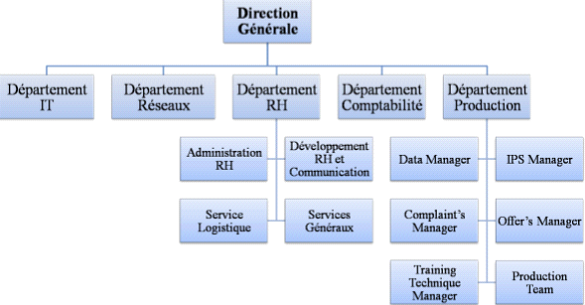
\includegraphics[width=0.8\textwidth]{./figures/Organigrammecmh.png}
    \caption{Organigramme de Mediassive}
    \label{fig:organigramme}
    \end{figure}
    
L'organisation de Mediassive repose sur une structure hiérarchique simple et efficace. La Direction Générale supervise la stratégie et les opérations de l'entreprise. Le Pôle IT \& Développement s'occupe du développement Web, mobile, blockchain et de la maintenance technique. Le Pôle Marketing Digital gère le SEO, les campagnes publicitaires, la gestion des réseaux sociaux et la stratégie de contenu. Le Pôle Design \& Communication se charge de l'identité visuelle, du UX/UI design et des supports multimédias. Enfin, le Support \& Assistance Client assure la relation client, le helpdesk et le suivi des projets.

\subsection{Services au Sein de l'Entreprise}

Mediassive propose une gamme complète de services incluant le marketing digital avec SEO, SEA et social media management. L'entreprise excelle également dans le développement Web et Mobile, ainsi que dans les solutions Web3 innovantes comprenant la blockchain, les smart contracts, les NFT et les dApps. Le design graphique et le branding font également partie de ses compétences, tout comme le consulting et la formation en stratégie digitale.

\section{Environnement de l'Entreprise}

\subsection{Clientèle}

La clientèle de Mediassive est variée et comprend principalement des startups technologiques, des entreprises locales souhaitant renforcer leur visibilité digitale, ainsi que des projets internationaux liés à la blockchain et au Web3.

\subsection{Fournisseurs}

L'entreprise collabore avec des fournisseurs de solutions numériques (hébergement cloud, outils analytiques, régies publicitaires en ligne, plateformes de développement).

\subsection{Concurrence}

Mediassive évolue dans un secteur compétitif où l'on retrouve des agences locales de communication digitale et des agences spécialisées en Web3 à l'international. Son atout réside dans son double positionnement : marketing digital classique et solutions Web3 innovantes.

\section{Présentation de l'Entreprise d'Accueil}

\subsection{À Propos de l'Entreprise}

Mediassive est une agence qui combine créativité, expertise digitale et technologies émergentes pour accompagner les entreprises dans leur développement numérique.

\subsection{Vision et Objectifs}

Mediassive aspire à être un acteur de référence dans le marketing digital et Web3 au Maroc et à l'échelle internationale. L'entreprise s'engage à promouvoir l'adoption des solutions blockchain et décentralisées, tout en contribuant activement à la digitalisation des entreprises locales.

\subsection{Locaux et Implantation}

L'entreprise est implantée à Laâyoune avec une présence au Technopark de Tanger, un espace favorisant l'innovation et la collaboration.
\section{Contexte et problématique}

\subsection{Contexte général}

Le marché du travail connaît aujourd’hui une transformation importante, marquée par le développement du freelancing, du travail à distance et des collaborations flexibles entre professionnels indépendants, entreprises et agences. Les organisations recherchent de plus en plus des profils qualifiés capables d’intervenir rapidement sur des missions spécifiques, tandis que les freelances souhaitent accéder à des opportunités adaptées à leurs compétences, à leur disponibilité, à leur localisation et à leurs préférences professionnelles.

Dans ce contexte, les plateformes de mise en relation jouent un rôle essentiel. Elles permettent de rapprocher les besoins des entreprises et des agences avec les compétences disponibles sur le marché. Cependant, les solutions existantes restent souvent limitées à une simple publication d’offres ou à une recherche manuelle de profils. Cette approche rend le processus parfois long, peu structuré et difficile à suivre.

FinderrLink s’inscrit dans cette logique de transformation digitale en proposant une plateforme web centralisée permettant de gérer les profils, les missions, les candidatures, les échanges, les notifications et les tableaux de bord. L’objectif est de faciliter la collaboration entre les différents acteurs tout en assurant une gestion claire des rôles et des permissions.

\subsection{Présentation des acteurs de la plateforme}

La plateforme FinderrLink repose sur plusieurs types d’utilisateurs ayant chacun des besoins et des droits spécifiques. Le freelance peut créer et gérer son profil professionnel, consulter les missions disponibles, postuler aux opportunités qui correspondent à son profil, sauvegarder des missions et suivre l’état de ses candidatures.

L’entreprise représente principalement un recruteur direct. Elle peut créer et publier des missions, gérer les candidatures reçues, consulter les profils freelances, sauvegarder des talents et entrer en contact avec les profils correspondant à ses besoins. Son rôle est donc orienté vers la recherche de compétences et la gestion des missions qu’elle propose.

L’agence possède un rôle plus flexible. Elle peut créer et gérer ses propres missions, comme une entreprise, mais elle peut également consulter les missions disponibles et y postuler, de manière similaire à un freelance. Cette particularité permet à l’agence d’agir à la fois comme recruteur pour ses propres besoins ou ceux de ses clients, et comme prestataire capable de répondre à des missions publiées sur la plateforme.

L’administrateur dispose d’un rôle de supervision. Il peut suivre l’activité globale de la plateforme, gérer les utilisateurs, contrôler les données principales et assurer le bon fonctionnement du système.

\subsection{Problématique de la fragmentation des informations}

L’un des principaux problèmes rencontrés dans le domaine du freelancing est la dispersion des informations. Les profils, les missions, les candidatures, les messages et les notifications sont souvent gérés à travers plusieurs outils ou plateformes distinctes. Cette fragmentation complique le suivi des activités, augmente le risque de perte d’information et ralentit les processus de recrutement et de collaboration.

Pour les freelances, cette situation rend la recherche de missions plus longue et moins efficace, car les opportunités ne sont pas toujours bien structurées ou adaptées à leur profil. Pour les entreprises, elle complique l’identification rapide des talents pertinents. Pour les agences, qui peuvent à la fois recruter et postuler à des missions, le besoin d’une gestion centralisée devient encore plus important.

Il est donc nécessaire de proposer une solution capable de regrouper l’ensemble des informations dans un environnement unique, clair et organisé.

\subsection{Problématique de la gestion des rôles et des accès}

Dans une plateforme regroupant plusieurs types d’utilisateurs, la gestion des droits d’accès constitue un enjeu essentiel. Les fonctionnalités accessibles ne doivent pas être identiques pour tous les utilisateurs. Un freelance ne doit pas avoir les mêmes permissions qu’une entreprise, une entreprise ne doit pas avoir les mêmes droits qu’une agence, et l’administrateur doit disposer d’un niveau d’accès plus avancé.

Cette diversité des rôles impose la mise en place d’un système RBAC, ou Role-Based Access Control. Ce système permet d’attribuer des permissions précises selon le rôle de chaque utilisateur. Il garantit que chaque acteur accède uniquement aux fonctionnalités qui correspondent à ses responsabilités.

Dans FinderrLink, cette logique est particulièrement importante, car l’agence possède un rôle hybride. Elle peut publier des missions comme une entreprise, mais elle peut également postuler à des missions comme un freelance. Le système de gestion des rôles doit donc être suffisamment précis pour prendre en charge ces différences fonctionnelles tout en maintenant la sécurité et la cohérence de l’application.

\subsection{Problématique du suivi des candidatures et de la communication}

Le suivi des candidatures représente un autre défi important. Les freelances ont besoin de connaître l’état de leurs candidatures, tandis que les entreprises et les agences doivent pouvoir organiser, analyser et traiter les candidatures reçues. Sans un outil structuré, ce suivi peut rapidement devenir complexe, surtout lorsque plusieurs missions et plusieurs profils sont gérés en même temps.

La communication entre les utilisateurs doit également être encadrée. Les échanges doivent respecter les règles métiers de la plateforme afin d’éviter les interactions non pertinentes ou non autorisées. La messagerie, les notifications et les statuts de candidature deviennent donc des éléments essentiels pour assurer une collaboration fluide et organisée entre les différents acteurs.

\subsection{Problématique liée à l’aide à la décision}

Un autre besoin important concerne l’aide à la décision. Les freelances peuvent avoir des difficultés à identifier les missions les plus adaptées à leur profil, surtout lorsque plusieurs opportunités semblent similaires. Les entreprises et les agences, de leur côté, peuvent rencontrer des difficultés à trouver rapidement les profils les plus pertinents parmi un grand nombre de freelances.

L’intégration d’un assistant intelligent permet de répondre à ce besoin en aidant les utilisateurs à rechercher des missions, comparer des opportunités, comprendre les détails d’une offre ou mieux exploiter les informations disponibles sur la plateforme. Cette dimension intelligente améliore l’expérience utilisateur et rend la plateforme plus efficace.

\subsection{Problème identifié}

Face à ces constats, le problème central peut être formulé ainsi :

\textbf{L’absence d’une plateforme centralisée, sécurisée et intelligente pour gérer la mise en relation entre freelances, entreprises et agences constitue un frein à l’efficacité du recrutement, au suivi des missions, à la gestion des candidatures et à la collaboration professionnelle.}

Une telle solution doit permettre de regrouper les profils, les missions, les candidatures, les échanges, les notifications et les tableaux de bord dans un seul environnement. Elle doit également intégrer une gestion précise des rôles, notamment pour distinguer les permissions du freelance, de l’entreprise, de l’agence et de l’administrateur.

Ainsi, FinderrLink vise à répondre à cette problématique en proposant une plateforme web complète, structurée et évolutive, capable d’améliorer la mise en relation entre les différents acteurs et de simplifier la gestion des processus liés aux missions professionnelles.
\section{Conclusion}

En conclusion, ce chapitre a permis de présenter le contexte général du projet FinderrLink, sa problématique ainsi que les objectifs visés. Le projet répond à un besoin réel de centralisation, de sécurité et d’efficacité dans la mise en relation entre freelances, entreprises et agences. Il s’inscrit également dans la vision de MEDIASSIVE, qui ne se limite pas aux services digitaux classiques, mais ambitionne aussi de développer et lancer ses propres solutions SaaS internes afin de répondre à des problématiques concrètes du marché.
